
%%% Local Variables:
%%% mode: latex
%%% TeX-master: t
%%% End:

\documentclass[12pt,a4paper,titlepage]{article}
\usepackage[style=numeric,backend=bibtex,firstinits=true,maxbibnames=99]{biblatex}
\usepackage{graphicx}
\usepackage{enumitem}
\usepackage{amssymb}
\usepackage[utf8]{inputenc}

\graphicspath{ {images/} }
\bibliography{report.bib}


\begin{document}

\begin{titlepage}

\newcommand{\HRule}{\rule{\linewidth}{0.5mm}} % Defines a new command for the horizontal lines, change thickness here

\center % Center everything on the page
 
\textsc{\LARGE University of Oxford}\\[1.5cm] % Name of your university/college
\textsc{\LARGE Honour School of Computer Science \\[0.2cm] and Philosophy}\\[0.5cm] % Major heading such as course name

\HRule \\[0.4cm]
{ \LARGE \bfseries Approximating Walrasian Equilibrium with Decentralized Bilateral Trade}\\[0.4cm] % Title of your document
\HRule \\[2cm]
 
\begin{minipage}{0.45\textwidth}
\begin{flushleft} \Large
\emph{Author:}\\
Victor Porras % Your name
\end{flushleft}
\end{minipage}
~
\begin{minipage}{0.45\textwidth}
\begin{flushright} \Large
\emph{Supervisor:} \\
Professor Paul Goldberg % Supervisor's Name
\end{flushright}
\end{minipage}\\[2cm]

{\Large {May 2017}}\\[2cm]

% \includegraphics[scale=0.2]{images/logo.png}
 
%----------------------------------------------------------------------------------------

\vfill % Fill the rest of the page with whitespace

\end{titlepage}

\begin{abstract}
  We simulate the convergence of a market with many traders through randomized bilateral trade.
\end{abstract}

\section{Introduction}
TODO: Brief outline of market and WE, why WE is important

The equilibrium conditions of markets have been widely studied in economics for hundreds of years.
In economics, a market is said to be in Walrasian equilibrium (WE) when no market participants can make any more profitable trades, and none of them subsidized each other. 
We will consider a market with m traders and n goods, where each trader begins with an endowment of some goods.
A Walrasian equilibrium (WE) is a set of prices and allocations of goods such that after every trader trades their endowment for their final allocation at those prices, they do not want to make any more trades.

The purpose of this project was to learn how algorithms like that in \cite{crockett} perform in practice.
TODO: more objectives

We investigate finding an approximate WE using decentralized bilateral trade.
In a given trading day, random pairs of traders make the largest trade possible until nobody can make any more trades. 
Following each day, the traders update constraints on the prices they are willing to accept.
After many days of tightening constraints, the market should converge to a stable set of prices and allocations, the approximate WE.
We implemented this algorithm in Python and experimented with different techniques of updating the constraints.

The naive implementation of this algorithm often failed to converge, and would instead diverge catastrophically, as the traders because overconstrained.
That made it unsuitable for finding the WE of a market.
To fix this, we developed a technique of backtracking to previous constraints with some probability when utilty fell below a threshold.
This made it possible to reliably simulate a market and obtain useful results.

We show that with backtracking, this algorithm finds approximate Walrasian equilibria consistently, and does not diverge.
We also show that the randomized algorithm gives the same results for a given endowment across multiple runs with different random numbers.
Lastly, we extend the algorithm to work without access to the gradient of the traders' utility functions.


The rest of this report is organized as follows.
Section~\ref{background} is an overview of the economic aspects of the project and its relation to previous work.
In Section~\ref{desimp}, we discuss the model we use and the choices we made when implementing it.
Section~\ref{results} contains the results we obtained from our simulations.
We analyze the success of the project and compare it to other methods in Section~\ref{conclusion}. 

\section{Background}\label{background}

This project focuses on simulating a world with two divisible goods that can be exchanged between a number of traders.
An assignment of goods to traders is called an \textit{allocation}.
Each trader in our world will receive a random initial \textit{endowment} allocation of goods, which they can trade with the others.
Thus, the allocation will change throughout a day of trading.

The \textit{marginal rate of substitution} between the two goods will be used throughout to represent price.
It applies to both potential and actual trades.
We always express the MRS and gradient (defined below) as units of good 2 per unit good 1.
For instance, a trade of 4 units of good 1 for 1 unit of good 2 has an MRS of 0.25.

The \textit{direction} of a trade is either ``Buy'' or ``Sell'', from the perspective of a given trader.
Direction is also expressed in terms of good 1, so a ``Buy'' means the trader is gaining good 1 by giving up good 2.
The direction is antisymmetric: a ``Buy'' for one trader is a ``Sell'' for their trading partner.

Utility functions capture the preferences of the actors in an economic model.
Utility is often associated with the pleasure or satisfaction that an actor gets from a situation.
A rational actor, by definition, always prefers an outcome with higher utility to one with lower utility. 
In general, a utility function is a function from states of the world to utilities.
In our case, it will be a function $\mathbb{R}^2_+ \rightarrow \mathbb{R}$ from the allocations of each good.

For this project, we use the Cobb-Douglas utility function:
\[
  u(x, y) = x^p y^{(1-p)}
\]
where x and y are the quantities of the goods.
TODO: rephrase this for clarity
Because this function is differentiable, we can calculate the gradient.
This makes it possible to calculate the slope of the line tangent to the function which is 
\[
  \frac{(1-p)y}{px}
\]

We will refer to the random number generator later in this report.
As in most applications, we actually use a \textit{pseudorandom} number generator.
This is a function which takes a \textit{seed} and produces a sequence of seemingly random numbers.
The crucial part is that the same seed will always produce the same sequence.
For other programs, the current time is often used as a seed so the sequence is not repeated.
However for our purposes, we will use specific seeds to get reproducible results and still reap the benefits of a randomized algorithm.

There is a long history of trial-and-error techniques in this field.
Walras' original idea for finding equilibrium is called tâtonnement, which means trial-and-error in French.
His approach was to have a centralized auctioneer pick a price, calculate the aggregate supply and demand, then adjust the price accordingly.
This seems very plausible, and it does work in practice for some special cases.

However, Scarf showed that there were initial allocations could be chosen so as to be unstable under this procedure \cite{scarf}.
Later research demonstrated that a modified tâtonnement procedure could be found, but only if the auctioneer has knowledge of all the traders' utility functions, including their gradients.

In the field, there are several different ways an equilibrium model can learn about the world. 
We use a utility oracle and a utility gradient oracle to access the preferences of two traders for a given allocation.
Significantly, the algorithm does not need to know anything about the whole system at once.
Another source is the aggregate demand oracle, which takes a vector of prices and gives the net supply and demand across the whole system.
This is what tâtonnement uses to find an equilibrium.

TODO: expand related work

Crockett, Spear, and Sunder investigate using trading to solve the divisible goods case \cite{crockett}.
They pioneer the use of constraints learned by traders to reach a WE and prove convergence guarantees for the two-trader case.
Unfortunately, they also show that there are cases where bilateral trade cannot find an exact equilibrium in the multitrader case.

Fleischer et al. give performance guarantees using an aggregate demand oracle to find approximate WE \cite{fleischer}.

Leme and Wong give a polynomial algorithm for the indivisible goods case using an aggregate demand oracle \cite{leme}.

In an unpublished note, Axtell and Goldberg suggested finding the quantitative performance of the algorithm suggested by Crockett, Spear, and Sunder \cite{goldberg}.
We have used this as our starting point.



\section{Design and Implementation}\label{desimp}
TODO: give little intro paragraph to design

\subsection{The Trading Day}

Each day of the simulation begins by giving each trader their initial endowment.
Then, pairs of traders are randomly selected to attempt a trade.
Each trader has access to their utility functions and the gradients of those functions for any allocation.
From the gradient and any constraints, we calculate two MRSs for each trader, one for each direction.
The direction of the potential trade (Trader1 buying from T2 or vice versa) is chosen based on the differences between their MRSs.
The trader with the higher MRS is the one who buys Good 1.
FIGURE diagram of trade.

In the standard model (see Section \ref{nograd} for the version without access to gradients), we calculate a joint MRS by taking the geometric mean of two MRSs.
This joint MRS is the exchange rate used for the potential.
We experimented with randomly picking an MRS between the two traders' MRSs, but this was slower and gave worse results.

TODO: paragraph on advantages of geometric mean

Then, we calculate the size of the biggest possible trade that can occur at that MRS.
A trade can occur if, after reallocation, both traders would have higher utilities.
We test progressively larger sizes, doubling each time.
Because the gradient only applies to infinitesimally small sizes, when the MRSs are very similar, the minimum size might not be possible.
If the largest size is non-zero, the traders exchange the appropriate goods and the process repeats.
Figure \ref{fig:day} shows a day of trading with three traders.

As we go, we keep track of the most recent MRS each trader agreed to trade at.
We use this later on to assess the quality of the simulation.

The simulation of a day ends once traders can make no more mutually beneficial trades.
To check for this, we track the number of consecutive attempted trades that are rejected. 
For a simulation with $n$ traders, we wait for $n$ consecutive such empty trades.
There is a parameter (--finish-count) that can increase or decrease this, but we found in practice that $n$ gives just as good results as $2n$ or $5n$, and is faster.

\begin{figure}[h]
    \centering
    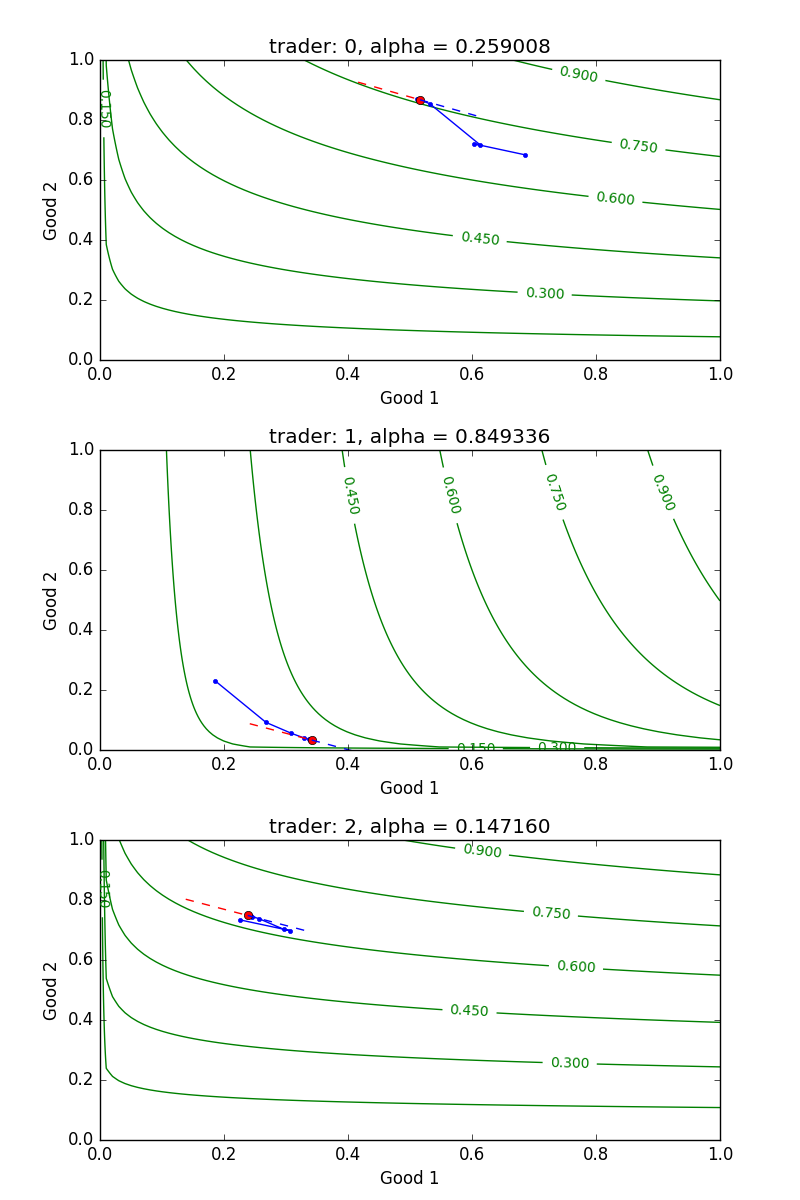
\includegraphics[width=\textwidth]{allocations_(seed_13).png}
    \caption{
      A single trading day for three traders.
      The green contours are lines of equal utility.
      Notice how the trades only increase utility.
      The red dots are the final positions of traders.
      TODO: explain dotted lines, all parallel
    }
    \label{fig:day}
\end{figure}

\subsection{Updating Constraints}
In order to have useful changes from one day to the next, the traders must change their behavior.
They achieve this by updating the constraints on the MRSs they will accept for buying and selling.

Using the definition of wealth from above, and the last MRS used globally, each trader calculates the wealth they gained or lost during the day.

Recall that no traders will accept trades that cause them to lose utility. 
Thus, we can calculate the non-negative utility gain by subtracting the utility of the initial endowment from the utility of the final allocation after a day's worth of trades.

First, if the trader updated their constraint from the previous day, they compare their wealth and utility gains from today to those from yesterday.
If the new constraint resulted in less utility or the same utility and less wealth, the constraint is reverted to its previous value.

When there was not a new constraint on the previous day or the constraint was successful, the trader considers tightening the constraint.
\begin{itemize}
  \item If they gained wealth during the day, they are happy with the MRSs they are accepting, so they don't make any changes.
  \item If they lost wealth, they determine whether they were a net buyer or seller of good 1.
  \item If they were a net buyer, they decrease their buying constraint, which is the highest price they will pay to buy good 1.
  \item If they were a net seller, they increase their selling constraint instead.
\end{itemize}
We will discuss the exact method of tightening in the evaluation section, when we compare different ones.

\subsection{Statistics}
At the end of each day, we calculate five statistics about the day's trading: These are used to evaluate the performance of the model.

The global utility gain, is the percentage increase in utility over the day for all the traders. 
Because it is a percentage, it can be compared across different starting allocations and numbers of traders.
It is supposed to increase over time then converge as the traders learn constraints that help them maximize their utility gains.

The wealth transfer is the sum of the absolute value of wealths gained or lost, divided by the total amount of wealth at the beginning.
Like above, it is marked to the last price that any trader trades at.
This should approach 0 over time.

As mentioned above, each trader has a most recent MRS they personally traded at.
In the ideal case, these all converge to the same value over the day, because if two traders disagree about MRS they can make a mutually beneficial trade.
To evaluate how close a simulation comes to this ideal, we calculate the standard deviation of the most recent MRS for each trader.
    
We record the average number of attempted trades per trader in the day.
We use this as our main method of comparing the running time of different models.
The elapsed clock time is also recorded, but this is less useful because it isn't comparable across machines.

Lastly, we calculate constrainedness based on the constraints used by each trader in the past day.
There are initial buy and sell constraints that every trader begins with.
This is the percentage of the original range between constraints that traders accept on average.
We actually use the log range, because the initial constraints vary by orders of magnitude and the plain range would underweight the lower (sell) constraint.
For example, constrainedness of 100\% means that 100\% of MRSs (within those initial constraints) are accepted.
Constrainedness of 5\% means that only 5\% of MRSs are acceptable on average.
We expect this to decrease over multiple days, and converge to a low value.

We track these statistics over many days of trading, and can analyze the results using a diagram like this.
This is a nice result, since all the stats do what we would expect.
We call this kind of outcome convergence.

\subsection{Convergence}
When designing models, we want to maximize the probabilty that they converge.
Convergence is a property of a trial of several days of trading.
Intuitively, as model converges when it stops getting better.
We define convergence as the point at which the average wealth transfer stops changing, with the caveat that the model does not meet the divergence criteria below.
More concretely, given a trial that has not diverged, the convergence point is the earliest day where the wealth transfer for all following days is within a threshold.
Experimentally, we have found that a threshold of 1\% seems to capture the examples that match the intuition above.

We defined convergence on wealth, not utility, because the utility was noiser and less like a monotone function.
Also, since the goal of this project is to approximate the output of an exact centralized system, we are trying to minimize wealth transfers.
It is possible that the ideal equilibrium actually has lower utility than the simulation, but the ideal wealth transferred is always zero.

For each model, we record the percentage of trials that converged, as well as the average wealth transfer, utility gain, MRS deviation, and constrainedness at that point.
We also record those same statistics at the end of the trial, though they are typically very similar.
The advantage of recording them at the end is that they can be compared across convergent and divergent cases.

\subsection{Divergence}
The biggest challenge in executing this project was avoiding divergence or death spiral.
A divergence is characterized by a decrease in utility and an increase in MRS deviation.
Figure \ref{fig:div} is a typical example of divergence. 
It is caused by the model becoming over-constrained, which leads to a reduction in trading volume.

We discovered this phenomenom when we tried the simpler models of constraint choice.
Every model would diverge in this manner on some trials, even after it had reached an acceptable state.
We wanted to avoid this in potential models, so we developed a criteria for identifying them automatically.

Formally, a trial is said to diverge if:
\begin{description}[align=right,labelwidth=2cm,font=\normalfont]
\item[1.] Utility gains fall at least 5\% from the first day 
\item[AND 2.] MRS deviation is greater than 0.1 
\end{description}
We use a moving average to smooth out condition 1.
    
To avoid divergence, we developed the technique of backtracking, which is discussed below.
TODO: expand here

\begin{figure}[h]
    \centering
    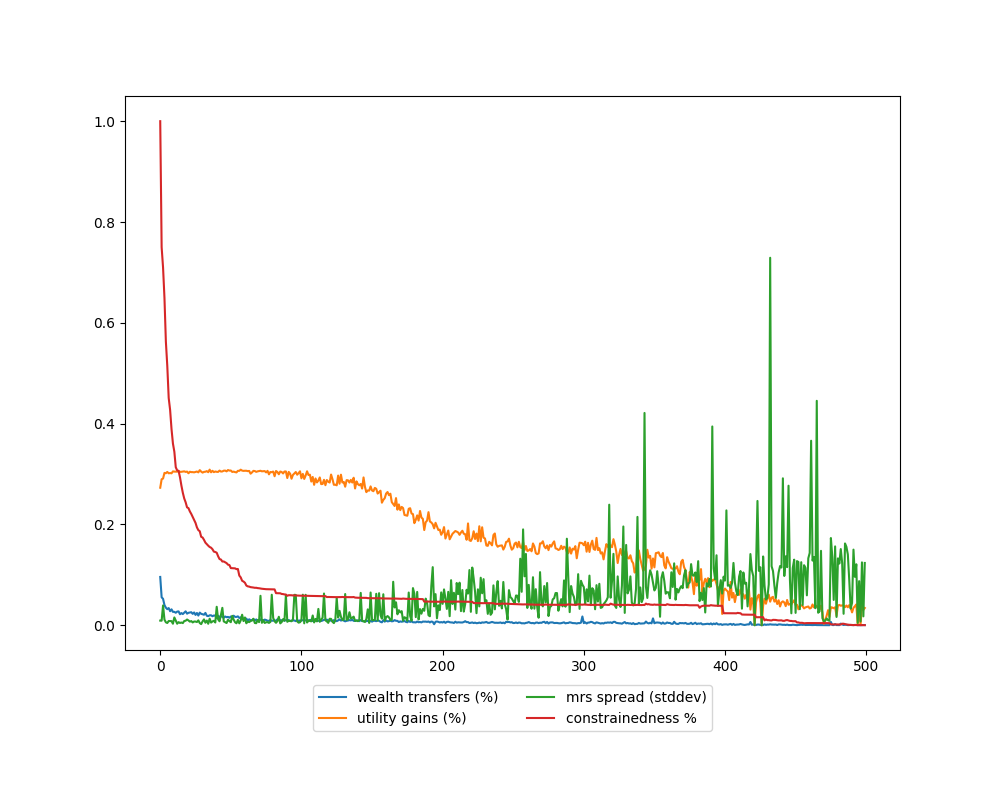
\includegraphics[width=\textwidth]{seed_0.png}
    \caption{
      Mean constraint with mean reversion, for 100 traders.
      Notice how utility falls around day 100 and MRS deviation increases dramatically.
    }
    \label{fig:div}
\end{figure}

\subsection{Testing}
Due to the wide parameter space and the length of time to construct experiments, we had to focus on analyzing some parameters, leaving others fixed.
We tested on models of 100 traders, because they showed the same dynamics as larger models, but still could be tested in only a couple of minutes per trial.
We ran each trial for 500 days, because most interesting things happened in days 50 to 150, and no model that we looked at diverged or converged after 500 rounds.

We tested 100 trials of each model, using different random allocations for each trial.
(Except for the stability experiments below)
However, we seeded the random number generator such that each model ran on the same set of endowments.
This means that any variations between models was not due to different endowments.
Multiple trials are necessary because the results are highly dependent on those endowments, which matches the intuition that the point of the project is to simulate economies with different endowments.
    
After the trials finished, the results were averaged to generate the summary statistics and the convergence/divergence rates.
For some models with 0\% convergence, the quality of convergence metrics are obviously not available.

\section{Results}\label{results}
\subsection{Simple Constraint Choice}
First, we investigated three ways of choosing restraints and three ways of reverting them.
The constraint choice is the action a trader takes when they lose wealth.
Reversion is when a constraint fails, and a trader needs to relax it.

Under fixed constraint choice, when a trader loses wealth, they contract their constraint by a fixed percentage.
This has the advantage of being simple to implement, and fast to evaluate.
It also would not require knowing the last MRS of the trader.
We tested this in three variations, with 5\%, 10\% and 20\% constraint factors.
For example, if the selling constraint was 5.0, a 10\% constraint factor would raise that to 5.5.
    
Last MRS constraint choice means that trader sets the constraint to the last MRS used.
This could lead to very quick convergence, because the trader would instantly adapt to the market price.

Mean constraint choice results in the trader setting the constraint to the geometric mean of the last price and the current constraint.
This moves more smoothly than last price and is more adaptive than fixed.

When a trader uses total reversion, they revert to the previous constraint when the current one fails.

Mean reversion is reverting to the geometric mean of the current constraint and the old constraint.
When combined with mean choice, it is equivalent to binary search over constraints.

Random reversion means that the trader reverts to a random MRS between the current constraint and the old constraint.

We tested all 15 combinations of constraint choice and reversion.
The full results are listed in TABLE.
The results were not particularly encouraging, with 77\% of trials diverging and only 15\% converging across the board.
Mean constraint choice was by far the most effective, with 63\% converging.
Mean choice with random reversion had 96\% convergence and only 1\% divergence.
However, it took almost three times as many trades to converge as mean-mean.
Mean-mean was efficient, but only converged 52\% of the time.
Total reversion was slower and less convergent than mean-mean.
All three had similar MRS divergence and utility gains at convergence.
Mean-random came out on top with only 3.7\% wealth transfers, a little ahead of mean-mean with 4.5\%.

Based on these results, we decided to focus on improving versions of the algorithm with mean constraint choice.

\subsection{Backtracking}

The main novel idea in this paper is the application of backtracking to this problem.
Backtracking means looking at past constraints, and if they gave better utility, switching to them with some positive probability.
The theoretical justification for this is that many variables are being optimized at once and many factors can affect the utility of a trader.
The trader's own actions, other traders' actions and randomness can all change the utility from day to day.
When a constraint is added initially, the trader keeps it they gain utility in the day immediately after.
However, it is possible that the supposed gain in utility actually came from other factors, and the constraint is negative in the long run.
It is also possible that the constraint might be good in the absence of other traders' behavior, but as they all adapt, the constraint ends up being too tight.
Thus, it sometimes might be the case that a constraint needs to be relaxed quite a bit to find the optimal solution.

To implement backtracking, each trader keeps track of their past utilities and constraint values.
They have a list of integers, called the "backtracks", which are relative indices used for comparison.
They also have a utility drop threshold and a backtrack probability.
At every day, they look backwards at their utility gains x days in the past for each x in their list of backtracks.
If their utility gain has fallen below the threshold since that day in the past, they will reset their constraint to what it was on that day with backtrack probability.

We tested a variety of different backtracks, probabilities and thresholds on a smaller trial size so we could try more combinations.
For all of the backtrack tests, we used mean constraint choice and mean reversion.
The specific locations of the backtracks did not seem to have much effect; for instance, backtracking at 4 is quite similar to backtracking at 9. 
Because of that, we ended up picking the values of 5, 25 and 100 to represent small, medium, and large backtracks, and only testing those.
The results from those are in APPENDIX.
From them, we selected a subset to run full size trials.
A 99\% threshold provided the highest quality results with no significant decrease in speed, so we use that level from here on.
We chose to run the full tests on probabilities of 50\%, 75\% and 100\%, and backtracks of 5, 25, 5-25 and 5-25-100. 

Overall, backtracking is a big improvement over the naive constraint choice.
The results are in TABLE.
Even the worst performing backtrack model had 83\% convergence and 16\% divergence.
The best model, with probability 50\% and backtracks at 5, 25, and 100 had 100\% convergence, with 34k average trades per trader until convergence.
Another model (just a single 25 backtrack) also had 100\% convergence, but was slower, with 49k trades until convergence.
The 50\%-5-25-100 model was only 29\% slower than the mean-mean model without backtracks, but it had much higher rate of convergence, and lower wealth transfers.

The high convergence percentage, with only 3.5\% wealth transfers and tight MRS convergence, makes this version of the algorithm a feasible approximation of the centralized methods. 
Backtracking greatly reduces the risk of divergence, which was the main issue in getting a decentralized program to be useful.

\subsection{Stability}
Stability is a desirable property for any random simulation of a event.
If the results are very sensitive to the seed of the random number generator, it casts doubt on whether the results reflect the parameters well.
In our case, we want to get the same results regardless of which pairs of traders are selected to trade.
To test this, we generated one set of starting allocations and ran many trials with different seeds on the same allocations.
We tried this with mean-mean in both convergent and divergent cases, as well as with the 50\%-5-25-100 backtracking model.

The results, in TABLE, show that the statistics are stable across different starting seeds.
The convergent allocations continued to converge 100\% of the time, and the divergent allocation did so 100\% of the time too.
It is encouraging that the best backtracking model remained stable, because that suggests that it could be safely used for simulating an allocation in practice.

\subsection{Convergence without Gradients}\label{nograd}
The system as described relies on the gradient of the utility function to choose a direction and MRS for attempted trades.
However, it is also possible to procede without the gradient and choose the direction and MRS randomly.
We can still use the constraints to define the range the MRS is chosen from.
Because of that, the traders will be able to learn the right MRS across multiple days of trading.
The trade sizing algorithm works fine with random price and direction, because the utilities of the traders can be queried as before, and the trade will only occur when it increases the utility for both.
The main effect of this is that many more trades must be attempted per success.

By giving up on differentiability, the model becomes closer to the real world, where people know their preferences but probably not the derivatives.
Additionally, it makes it possible to use a wider variety of utility functions, especially piecewise linear ones which are important in the literature \cite{chen}.
There is even the possibility of using non-deterministic utility functions, where the utility function samples a probability distribution.
This would work fine with the relaxed model as long as the queries were deterministic within individual trades.
(eg if the oracle says a trade is plus-utility, and so it is accepted, then it must lead to a gain in utility, even if the same terms are rejected on another day) 

We tested this with the mean-mean constraint model.
To get it to work, we had to adjust a few parameters. 
First, we changed the minimum trade size from 0.0001 to 0.0000001 
Note that since the sizes expand geometrically as long as they are plus-utility, this is only $\log_2 1000$ more steps per trade, rather than 1000.
We also increased the finish count from 1 to numbers between 5 and 30.
This meant that the model would wait for more empty trades before finishing a day.
This was necessary because the ratio of successful to empty trades is so much lower.
These changes are appropriate because this algorithm is so much simpler and faster already that it still ran faster than the normal model after the modifications.

After testing on a variety of finish counts, we can conclude that
TODO: this

\section{Conclusion}\label{conclusion}

\subsection{Achievements}
This project is a step towards better calculation of Walrasian equilibria via bilateral trade.
We implemented a simulation framework that can test different models of constrained bilateral trade.
We addressed a significant issue with the constraint-learning method of calculation with the novel addition of backtracking.


\subsection{Evaluation}
The main advantage of the techniques in this project over the existing methods available is that the information requirements are much lower. 
We do not assume that there is a central auctioneer who can query everyone's preferences at the same time.
This would be unrealistic in many real world markets.

We unfortunately do not have an easy way of comparing the efficiency of the two since we did not test the centralized methods on the same hardware, and our metric of attempted trades does not apply to a deterministic approach.

We can say that our approach is linear in the number of traders. 
This is supported experimentally by running experiments on different numbers of traders.
The results for the mean-mean simulation on 50 to 500 traders are displayed in TABLE.
This reflects the intuition that more traders doesn't change the average number of trades a given trader must interact with.
Because the trading pairs were randomized to begin with, a trader is indifferent to where the others traders come from.

TODO: expand and cite


\subsection{Future Work}
It would be very useful to compare this directly to the centralized ways of calculating Walrasian equilibria.
In particular, the utility gains from the actual equilibrium could be compared with the simulated results.
If it was implemented in the same language, running time could also be compared in practice.

We only focused on the very simple case of two goods.
Every centralized model supports more goods, which is more realistic.
We believe this could be expanded to more goods, but it would take a substantial change to the code and was such outside the scope of the project.

We would like to test our model against a wider variety of utility functions, since it theoretically has the capability to simulate them.


\section{Acknowledgements}\label{acknowledgements}
I would like to thank my supervisor, Paul Goldberg for giving me the idea for the project and all his advice along the way.

% I would also like to thank my tutor, Prof. Thomas Melham for reviewing a draft of this report.

\printbibliography

\end{document}

%%% Local Variables:
%%% mode: latex
%%% TeX-master: t
%%% End:
